% !TEX TS-program = XeLaTeX
% use the following command:
% all document files must be coded in UTF-8
\documentclass[spanish]{textolivre}
% build HTML with: make4ht -e build.lua -c textolivre.cfg -x -u article "fn-in,svg,pic-align"

\journalname{Texto Livre}
\thevolume{16}
%\thenumber{1} % old template
\theyear{2022}
\receiveddate{\DTMdisplaydate{2022}{10}{24}{-1}} % YYYY MM DD
\accepteddate{\DTMdisplaydate{2022}{12}{7}{-1}}
\publisheddate{\DTMdisplaydate{2023}{1}{13}{-1}}
\corrauthor{Angélica Montaner Henríquez}
\articledoi{10.1590/1983-3652.2023.41570}
%\articleid{NNNN} % if the article ID is not the last 5 numbers of its DOI, provide it using \articleid{} commmand 
% list of available sesscions in the journal: articles, dossier, reports, essays, reviews, interviews, editorial
\articlesessionname{dossier}
\runningauthor{Montaner Henríquez y Ambrós-Pallarés} 
%\editorname{Leonardo Araújo} % old template
\sectioneditorname{Hugo Heredia Ponce}
\layouteditorname{Daniervelin Pereira}

\title{Expansión transmedia de un cuento para desarrollar la interpretación literaria}
\othertitle{Expansão transmídia de uma história para desenvolver a interpretação literária}
\othertitle{Transmedia expansion of a story to develop literary interpretation}
% if there is a third language title, add here:
%\othertitle{Artikelvorlage zur Einreichung beim Texto Livre Journal}

\author[1]{Angélica Montaner Henríquez~\orcid{0000-0003-1352-8544}\thanks{Email: \href{mailto:angelicamontaner.h@gmail.com}{angelicamontaner.h@gmail.com}}}
\author[2]{Alba Ambrós-Pallarés~\orcid{0000-0002-4450-2067}\thanks{Email: \href{mailto:aambrosub@gmail.com}{aambrosub@gmail.com}}}
\affil[1]{Escuela Diego Portales, San Bernardo, Región Metropolitana, Chile.}
\affil[2]{Universidad de Barcelona, Barcelona, España.}

\addbibresource{article.bib}
% use biber instead of bibtex
% $ biber article

% used to create dummy text for the template file
\definecolor{dark-gray}{gray}{0.35} % color used to display dummy texts
\usepackage{lipsum}
\SetLipsumParListSurrounders{\colorlet{oldcolor}{.}\color{dark-gray}}{\color{oldcolor}}

% used here only to provide the XeLaTeX and BibTeX logos
\usepackage{hologo}

% if you use multirows in a table, include the multirow package
\usepackage{multirow}

% provides sidewaysfigure environment
\usepackage{rotating}

% CUSTOM EPIGRAPH - BEGIN 
%%% https://tex.stackexchange.com/questions/193178/specific-epigraph-style
\usepackage{epigraph}
\renewcommand\textflush{flushright}
\makeatletter
\newlength\epitextskip
\pretocmd{\@epitext}{\em}{}{}
\apptocmd{\@epitext}{\em}{}{}
\patchcmd{\epigraph}{\@epitext{#1}\\}{\@epitext{#1}\\[\epitextskip]}{}{}
\makeatother
\setlength\epigraphrule{0pt}
\setlength\epitextskip{0.5ex}
\setlength\epigraphwidth{.7\textwidth}
% CUSTOM EPIGRAPH - END

% LANGUAGE - BEGIN
% ARABIC
% for languages that use special fonts, you must provide the typeface that will be used
% \setotherlanguage{arabic}
% \newfontfamily\arabicfont[Script=Arabic]{Amiri}
% \newfontfamily\arabicfontsf[Script=Arabic]{Amiri}
% \newfontfamily\arabicfonttt[Script=Arabic]{Amiri}
%
% in the article, to add arabic text use: \textlang{arabic}{ ... }
%
% RUSSIAN
% for russian text we also need to define fonts with support for Cyrillic script
% \usepackage{fontspec}
% \setotherlanguage{russian}
% \newfontfamily\cyrillicfont{Times New Roman}
% \newfontfamily\cyrillicfontsf{Times New Roman}[Script=Cyrillic]
% \newfontfamily\cyrillicfonttt{Times New Roman}[Script=Cyrillic]
%
% in the text use \begin{russian} ... \end{russian}
% LANGUAGE - END

% EMOJIS - BEGIN
% to use emoticons in your manuscript
% https://stackoverflow.com/questions/190145/how-to-insert-emoticons-in-latex/57076064
% using font Symbola, which has full support
% the font may be downloaded at:
% https://dn-works.com/ufas/
% add to preamble:
% \newfontfamily\Symbola{Symbola}
% in the text use:
% {\Symbola }
% EMOJIS - END

% LABEL REFERENCE TO DESCRIPTIVE LIST - BEGIN
% reference itens in a descriptive list using their labels instead of numbers
% insert the code below in the preambule:
%\makeatletter
%\let\orgdescriptionlabel\descriptionlabel
%\renewcommand*{\descriptionlabel}[1]{%
%  \let\orglabel\label
%  \let\label\@gobble
%  \phantomsection
%  \edef\@currentlabel{#1\unskip}%
%  \let\label\orglabel
%  \orgdescriptionlabel{#1}%
%}
%\makeatother
%
% in your document, use as illustraded here:
%\begin{description}
%  \item[first\label{itm1}] this is only an example;
%  % ...  add more items
%\end{description}
% LABEL REFERENCE TO DESCRIPTIVE LIST - END


% add line numbers for submission
%\usepackage{lineno}
%\linenumbers


\begin{document}
\maketitle

\begin{polyabstract}
\begin{abstract}
El objetivo de esta investigación es describir la función didáctica de la expansión transmedia de un cuento para el desarrollo de la interpretación literaria. Para ello se diseñó e implementó una secuencia didáctica orientada a la producción de narrativas transmedia del cuento “Bocas cosidas”, realizada por docentes en Chile durante el período de confinamiento, en el año 2020. La metodología empleada es la sistematización de experiencias y el análisis temático de las creaciones. Los resultados demuestran que la producción transmedia contribuye al desarrollo de la interpretación literaria. Los indicadores tomados en cuenta fueron la definición del tema de las narrativas transmedia, la expansión del mundo narrativo del cuento, los elementos audiovisuales empleados, las alusiones a su intertexto lector y las relaciones de intertextualidad establecidas.

\keywords{Innovación pedagógica \sep Método de aprendizaje \sep Enseñanza multimedia \sep Análisis literario \sep Escritura creativa}
\end{abstract}

\begin{portuguese}
\begin{abstract}
O objetivo desta pesquisa é descrever a função didática da expansão transmídia de uma história para o desenvolvimento da interpretação literária. Para isso, foi idealizada e implementada uma sequência didática voltada para a produção de narrativas transmídia da história “Bocas cosidas”, realizado por professores no Chile durante o período de confinamento, em 2020. A metodologia utilizada é a sistematização de experiências e a análise temática das criações. Os resultados mostram que a produção transmídia contribui para o desenvolvimento da interpretação literária. Os indicadores levados em consideração foram a definição do tema das narrativas transmídia, a ampliação do mundo narrativo da história, os elementos audiovisuais utilizados, as alusões ao seu intertexto de leitura e as relações de intertextualidade estabelecidas.

\keywords{Inovação pedagógica \sep Método de aprendizagem \sep Educação multimídia \sep Análise literária \sep Escrita criativa}
\end{abstract}
\end{portuguese}

\begin{english}
\begin{abstract}
The objective of this research is to describe the didactic function of the transmedia expansion of a story for the development of literary interpretation. To this end, a didactic sequence was designed and implemented oriented to the production of transmedia storytelling of the story “Bocas cosidas”, carried out by teachers in Chile during the lockdown, in 2020. The methodology used is the systematization of experiences and the thematic analysis of the creations. The results show that transmedia production contributes to the development of literary interpretation. The indicators taken into account were the definition of the theme of transmedia storytelling, the expansion of the narrative world of the story, the audiovisual elements used, the allusions to their reading intertext and the relations of intertextuality established.

\keywords{Teaching method innovations \sep Learning methods \sep Multimedia instruction \sep Literary analysis \sep Creative writing}
\end{abstract}
\end{english}
% if there is another abstract, insert it here using the same scheme
\end{polyabstract}

\section{Introducción}\label{sec-intro}
La interpretación literaria es una de las habilidades clave que predomina en las Bases Curriculares de Lengua y Literatura en Chile \cite{ministerio_de_educacion_bases_2015,ministerio_de_educacion_bases_2019}. Dicha habilidad involucra una serie de conocimientos ligados a la educación literaria, tales como el reconocimiento de relaciones intertextuales, activación del intertexto lector, conciencia del contexto de producción y reproducción, entre otros \cite{mendoza_fillola_lectura_1995,mendoza_fillola_tu_1998,ministerio_de_educacion_bases_2019}. 

Sin embargo, pese a la importancia que se otorga a esta habilidad, los resultados del país en pruebas estandarizadas de competencia lectora como PISA demuestran que su desarrollo aun es deficitario, obteniendo un resultado menor –452 puntos–, al promedio de la OCDE – 487 puntos– \cite{agencia_de_calidad_de_la_educacion_pisa_2019}. 

Este resultado se podría asociar a que en la actualidad no existe uniformidad en la implementación de procesos de enseñanza-aprendizaje destinados al desarrollo de la competencia lecto-literaria, desembocando en una diversidad de estrategias desplegadas en las clases de educación literaria, entre las que se encuentran aquellas de carácter análogo, y otras del ámbito digital \cite{suazo_munoz_aproximacion_2022}. 

Lo expuesto anteriormente, resulta contraproducente con las Bases Curriculares en tanto que promueven el desarrollo de las habilidades del siglo XXI, específicamente las de alfabetización digital. Dicha alfabetización contempla, por un lado, el manejo de las herramientas de trabajo que ofrece la tecnología, junto con su uso creativo e innovador; y, por otro lado, la creatividad e innovación, que implica tanto la imitación de contenidos, como la creación original de estos \cite{ministerio_de_educacion_bases_2019}.  

El contexto vivido de la pandemia y post pandemia enfatiza la necesidad de desarrollar estas habilidades para la implementación de la tecnología en educación, tanto a nivel de docentes como de discentes. Sin embargo, las investigaciones en torno a la competencia digital de los agentes educativos desplegadas desde la Covid-19 y el consecuente cierre de los establecimientos educativos, han evidenciado que su desarrollo está en un proceso inicial, dificultando la integración de las TIC para el diseño de experiencias significativas de aprendizaje \cite{ramos-pla_formacion_2022,aguilar_cuesta_covid-19_2022,guillen-gamez_formacion_2022,area_tecnologias_2021}.

En el ámbito específico de la didáctica de la literatura, se identifica que a los profesores del área les ha dificultado integrar el uso didáctico de las TIC para la educación literaria. Sin embargo, quienes lo han hecho, ha sido más bien intuitivamente, debido a la escaza o nula capacitación que recibieron en su formación inicial docente \cite{suazo_munoz_aproximacion_2022,gonzalez_integracion_2018}. 

Tomando en consideración las premisas anteriores, surge el interrogante de cómo podría contribuir el uso de la tecnología y las habilidades de alfabetización digital al desarrollo de la interpretación literaria. Para responder a ello, se diseñó una secuencia didáctica, destinada en primera instancia a estudiantes, no obstante, por la aparición de la pandemia no se les pudo aplicar, por lo que se invitó a participar a cuatro docentes de Lengua y Literatura, para indagar sobre las posibilidades didácticas de la expansión narrativa, mediante la producción de narrativas transmedia, con el fin de mejorar la interpretación literaria \cite{ballester_roca_clasicos_2021}.

El objetivo general de la investigación consiste en describir la función didáctica de la expansión transmedia para el desarrollo de la interpretación literaria, mediante la producción de narrativas transmedia del cuento “Bocas cosidas” \cite{barros_bocas_2015}, en el marco de una secuencia didáctica denominada \#AntologíaNarrativaTransmedia, creada ad hoc para este estudio. 

\section{Marco teórico}\label{sec-normas}
La educación literaria se define como un “conjunto de saberes que permiten leer e interpretar un texto” \cite[p. 71]{mendoza_fillola_educacion_2004}, desarrollando en los estudiantes aprendizajes que les permiten acceder y realizar lecturas cada vez más complejas \cite{jover_educacion_2010}. En esta definición, la interpretación se enmarca como un aspecto clave en la educación literaria, en tanto posibilita la construcción de significados nuevos, incluso de obras que ya han sido leídas a lo largo de diferentes épocas.  

\subsection{Interpretación literaria}\label{sec-conduta}
La interpretación literaria se entiende en este estudio como un proceso en el que se otorga sentido a un texto, mediante la interacción entre su contenido, los saberes del lector, su visión del mundo, el propósito perseguido por la obra y por el lector, además de los contextos de producción y de recepción \cite{mendoza_fillola_lectura_1995,mendoza_fillola_tu_1998}. Todo ello confluye en el intertexto lector, es decir, en el espacio donde convergen los diversos saberes que se activan en la conciencia del lector por requerimiento de un texto \cite{garagalza_sentido_2014}. La definición se enmarca en el denominado modelo lector, que promueve la adquisición de la competencia lecto-literaria, entendiendo que: 

\begin{quote}
    La obra es también la experiencia del lector (Pragmática, Teoría de la Recepción) desde el momento en que éste debe completar los elementos no dichos, los lugares de indeterminación, o anticipar hipótesis y conjeturas sobre las mismas en el marco de la historia de la recepción de dichas obras y de su relación con las normas estéticas y las expectativas que posibilitan su lectura en diferentes épocas \cite[p. 30]{nunez_molina_modelos_2016}.
\end{quote}

En este contexto, la interpretación literaria funciona como un ejercicio creativo en el que se proponen nuevos sentidos para un mismo texto, en virtud de los conocimientos previos del lector y del momento en que fue leído \cite{ministerio_de_educacion_bases_2019}. Ello no significa que todas las interpretaciones sean adecuadas, esto se medirá a partir de la coherencia que mantenga con el texto base, para lo cual se requiere de una lectura atenta, reflexiva y de un análisis exhaustivo de la obra. Ahora bien, cabe pensar cómo se lleva a cabo este proceso de interpretación literaria en las clases de Lengua y Literatura, frente a lo cual se identifican diversas técnicas como el análisis literario y el comentario del texto \cite{cassany_taller_2006}, técnicas que implican principalmente el uso escrito y oral de la lengua. 

Fruto de la experiencia como docente de lengua y literatura en el aula de seis años en Chile, y de las nuevas perspectivas del currículo del MINEDUC para este ámbito, surge la pregunta de investigación de cómo se desarrollará la interpretación literaria si empleamos herramientas digitales para construir el sentido que otorgamos a una obra; y si esta se verá influenciada por el escaso nivel de desarrollo de la competencia digital docente \cite{suazo_munoz_aproximacion_2022,ramos-pla_formacion_2022,aguilar_cuesta_covid-19_2022,guillen-gamez_formacion_2022,area_tecnologias_2021,gonzalez_integracion_2018}.

\subsection{Expansión transmedia de una obra literaria}\label{sec-fmt-manuscrito}
Diversos estudios hablan de la función didáctica de las TIC para la educación literaria, sin embargo, su uso se ha limitado al fomento lector, dejando de lado su utilidad para el desarrollo de la interpretación literaria \cite{margallo_gonzalez_educacion_2012}. Esta idea se asocia a lo expuesto por \textcite{aguilar_cuesta_covid-19_2022} con relación a la competencia digital docente, cuya dimensión de creatividad e innovación es la de menor dominio, dentro de la cual se encuentran los descriptores “Ideas originales con TIC” y “Creación de recursos”.

Frente al desafío de emplear las TIC para profundizar la interpretación literaria de una obra, se optó por elegir la denominada Narrativa Transmedia (NT) que corresponde a un texto multimodal y multimedia que expande el mundo narrativo de un texto, a través de diversos formatos y múltiples plataformas \cite{jenkins_convergence_2006,scolari_narrativas_2013,kalogeras_transmedia_2014,scolari_transmedia_2018}. Además, conlleva una metodología activa que motiva a profesorado y alumnado \cite{hernandez-ortega_metodologias_2021}. El punto de partida es un texto base, cuyo universo narrativo se extiende a partir de diversas producciones conectadas a él. En consecuencia, no se trata de una adaptación del hipotexto a otros formatos, sino de nuevas creaciones a partir de él, respetando los elementos clave del mundo narrativo que lo componen, posicionándose como “una práctica de producción de sentido e interpretativa basada en historias que se expresan a través de una combinación de lenguajes, medios y plataformas” \cite[p. 25]{scolari_narrativas_2013}.

Dada la riqueza interpretativa de las NT, se ha propuesto en esta investigación que las docentes de Lengua y Literatura hagan la expansión transmedia de un cuento. Para su implementación, \cite{ramos_estrategias_2008} proponen emplear la transcodificación que consiste en una “operación o conjunto de operaciones, por la que un elemento o un conjunto significante se traslada de un código a otro, de un lenguaje a otro lenguaje” \cite[p. 72]{mendoza_fillola_tu_1998}. Todas estas acciones promueven el desarrollo de la interpretación literaria a través de las decisiones que toma el lector al escoger los significantes más adecuados para el significado asociado al texto. Ello es posible a partir del análisis de la obra y de la activación del intertexto lector durante su ejecución, puesto que es el que permite establecer conexiones entre la obra, las experiencias vitales del lector, y su conocimiento de diversas producciones artísticas y culturales. 

La selección del cuento “Bocas cosidas” para llevar a cabo la expansión transmedia de su universo narrativo, obedece tanto a su riqueza simbólica, reflejada en las metáforas empleadas a lo largo de la historia, como a la temática feminista planteada por Barros y su conexión con el intertexto lector de las participantes de este estudio. Su prosa se caracteriza por dos ejes fundamentales, la denuncia de la violencia física y simbólica sustentada en las relaciones de poder y sumisión que se establecen entre hombres y mujeres; y la transgresión a lo que socialmente se entiende como femenino, bajo el alero de un sistema patriarcal \cite{asensio_erotismo_2016,moreno_ramos_artemisa_2014,lobos_martinez_pibarros:_2013}.


\subsection{Secuencia didáctica}\label{sec-formato}
La secuencia didáctica (SD) es una metodología activa de enseñanza-aprendizaje, en la que se articulan actividades de aprendizaje de lectura y de escritura, de evaluación y de metacognición, en torno a uno o más textos. En esta, los usuarios ponen en práctica una serie de conocimientos, habilidades y actitudes en función de la elaboración de un producto final, que contempla los objetivos de aprendizaje establecidos para la SD \cite{dolz_sexprimer_2001,camps_secuencias_2003,ramos_estrategias_2008,tobon_tobon_secuencias_2010,correro_educacion_2016}.

En el ámbito de la didáctica de la lengua y la literatura, se ha propuesto la SD en forma de proyectos, orientados al aprendizaje de la escritura y al desarrollo de la educación literaria \cite{camps_secuencias_2003,correro_educacion_2016}, abarcando así:

\begin{quote}
    Actividades de lectura y de escritura, por lo que los alumnos son receptores, pero a la vez emisores de mensajes orales y escritos. Estos mensajes pueden tener un carácter reflexivo u organizativo del conocimiento o, en determinados casos, un valor creativo. \cite[p. 145]{ramos_estrategias_2008}
\end{quote}

Existe un modelo de SD, impulsado por \textcite{camps_secuencias_2003}, que contempla tres fases: preparación, realización y evaluación, el que se ha tomado como referente para el diseño de la SD creada para esta investigación. 

En la \textbf{fase de preparación} se deciden las características del proyecto, las tareas que se ejecutarán y los objetivos de aprendizaje. En la \textbf{fase de realización} están las actividades de aprendizaje, las cuales se pueden dividir en tres tipos: las actividades de lectura, las actividades de producción y las actividades destinadas a conocer las características formales del texto a elaborar. La última fase corresponde a la \textbf{evaluación de la producción} de la SD, la cual no solo ocurre una vez finalizada, sino que está presente a lo largo de todo el proceso a través de las actividades de metacognición.

Para la SD elaborada en el marco de esta investigación, se ha incluido dentro de la fase de realización actividades de lectura, de interpretación y de producción, empleando para ello el análisis literario, el comentario del texto \cite{cassany_taller_2006}, la transcodificación \cite{mendoza_fillola_tu_1998,ramos_estrategias_2008} y la expansión transmedia para la creación de una NT de la interpretación literaria de una obra. 

\section{Método}\label{sec-modelo}
En este estudio se emplea el análisis de contenido para valorar la función didáctica de la expansión transmedia de un cuento, a partir de los procesos llevados a cabo por las participantes del estudio, profundizando en sus puntos de vista e interpretaciones \cite{hernandez_metodologiinvestigacion_2014}. A su vez, la metodología empleada es la sistematización de experiencias, pues se centra en la descripción e interpretación crítica de los procesos que se desarrollaron en las etapas de una experiencia, con el propósito de extraer aprendizajes de ella \cite{oscar_sistematizacion_2018}.

La experiencia sistematizada es el proceso de interpretación literaria llevado a cabo por las docentes, en el marco de la SD \#AntologíaNarrativaTransmedia creada para esta investigación (\Cref{tab01}), constituyéndose como eje de sistematización la función didáctica de la expansión transmedia para el desarrollo de la interpretación literaria.

\subsection{Instrumento}\label{sec-organizacao}
La SD creada\footnote{En el siguiente enlace se encuentra la SD creada para esta investigación \url{https://doi.org/10.6084/m9.figshare.21383547.v2}} es el instrumento principal de recogida de datos, cuya versión preliminar se contrastó con dos expertos del área. Está compuesta de seis sesiones de una duración aproximada de 13 horas, en las que las cuatro docentes tuvieron que leer el cuento “Bocas cosidas”\footnote{El cuento se puede leer a través de la página web del diario digital de crítica cultural en Sudamérica, Cine y Literatura: \url{https://www.cineyliteratura.cl/bocas-cocidas-cuento-pia-barros/}}, desarrollar un análisis interpretativo de él, realizar un protocolo de escritura y producir una NT, a partir de la interpretación literaria realizada. Al mismo tiempo, se llevaron a cabo dos grupos de enfoque destinados a compartir las interpretaciones literarias formuladas y a reflexionar sobre los aprendizajes desarrollados a partir de la realización de las actividades.

\begin{table}[h!]
\centering \small
\begin{threeparttable}
\caption{SD \#\textit{AntologíaNarrativaTransmedia}.}
\label{tab01}
\begin{tabular}{
    >{\raggedright\arraybackslash}p{2cm} 
    >{\raggedright\arraybackslash}p{2.5cm} 
    >{\raggedright\arraybackslash}p{1.2cm} 
    >{\raggedright\arraybackslash}p{2cm} 
    >{\raggedright\arraybackslash}p{1.5cm} 
    >{\raggedright\arraybackslash}p{1.5cm} 
    >{\raggedright\arraybackslash}p{1.5cm}
    }
\toprule
 \textbf{Sesiones de la SD} & \textbf{Objetivo} & \textbf{Fecha} & \textbf{Instrumento de recogida de datos} & \textbf{Formato de recogida de los datos} & \textbf{Plataforma de recogida de datos} & \textbf{Análisis de los datos} \\
 \midrule
1.Análisis interpretativo del cuento “Bocas cosidas” (2015)
& Formular una interpretación literaria del cuento “Bocas cosidas” (2015) y explicar los pasos realizados para esto. &
06 de mayo de 2020 & SD: guía de trabajo Nº 1 & Escrito & Correo electrónico & Análisis temático \\
2.Compartiendo nuestras interpretaciones literarias & Compartir y evaluar las interpretaciones elaboradas del cuento. & 09 de mayo de 2020 & SD: grupo de enfoque  & Audio & \textit{Jitsi Meet} & Análisis temático \\
3. Protocolo de escritura: planificación de la NT & Planificar la producción de una NT sobre su interpretación del cuento, a través de un protocolo de escritura. & 20 de mayo de 2020 & SD: protocolo de escritura & Escrito & Correo electrónico & Análisis temático \\
4. Protocolo de escritura: producción de la NT & Producir la NT de su interpretación literaria, utilizando las TIC, creativamente. & 20 de mayo de 2020 & SD: protocolo de escritura  & Escrito & Correo electrónico & Análisis temático \\
5. Protocolo de escritura: producción digital de la NT & Producir la NT de su interpretación literaria, a través del programa digital escogido. & 12 de junio de 2020 & SD: NT digitales  & Audiovisual & Correo electrónico & Análisis temático \\
6. Reflexión sobre el proceso de interpretación literaria a través de una NT & Reflexionar y evaluar el proceso de interpretación literaria a través de la creación de una NT. & 14 de julio de 2020 & SD: grupo de enfoque & Audio & Jitsi Meet & Análisis temático \\
\bottomrule
\end{tabular}
\source{Elaboración propia.}
\end{threeparttable}
\end{table}

\subsection{Participantes}\label{sec-organizacao-latex}
Participaron de este estudio cuatro profesoras chilenas de Lengua y Literatura en educación secundaria, desempeñándose en establecimientos públicos y particulares subvencionados, contando con dos años de experiencia docente en aula como mínimo. 

Su titulación es de Pedagogía en Castellano, de la Universidad de Playa Ancha y satisfacían tres criterios definidos en la investigación: en primer lugar, se requería que su grado fuese especializado en educación de Lengua y Literatura; en segundo lugar, que se desempeñaran en la asignatura de Lengua y Literatura del Currículo Escolar; y, en tercer lugar, que contaran con el tiempo y voluntad para desarrollar la SD.

Se contactó con ellas –Amelia, Gladys, Ester y Tamara– vía correo electrónico, indicándoles el propósito del estudio, y una vez aceptada la participación, se les informó del código ético de protección de datos\footnote{Amelia, Gladys, Ester y Tamara es una identificación ficticia para mantener el anonimato de las profesoras, según lo indicado en el código ético europeo de protección de datos para la integridad y honestidad en la investigación, empleado por la Federación Europea de las Academias de las Ciencias y Humanidades \cite{all_european_academies_allea_codigo_2018}.}.

\subsection{Análisis}\label{sec-titulo}
Una vez recogidas las respuestas escritas, las grabaciones de los dos grupos de enfoque y las NT creadas por las docentes en el marco de las actividades de la SD, se codificó y transcribió su contenido\footnote{Los nombres ficticios de Amelia, Gladys, Ester y Tamara fueron empleados para la codificación. En las citas textuales del discurso de las docentes, superiores a 40 palabras, se ha indicado la inicial del nombre, más la inicial, “A6”, que corresponde al apartado de transcripciones de la investigación, y el número de línea de la transcripción, por ejemplo “A\_A6\_213-218”. La transcripción de las actividades de la SD desarrolladas por las docentes fue de tipo literal, y la transcripción de los grupos de enfoque fue ortográfica. Ello con el propósito de ser consecuentes con el análisis temático empleado en este estudio y con los resultados esperados.}.

Para el tratamiento de los datos se empleó el análisis temático \apud{braun_using_2006}{mieles_barrera_investigacion_2012}, 
a partir del eje de sistematización del estudio, que en la investigación previa correspondía al proceso de interpretación literaria de las docentes, sin embargo, por el propósito de este estudio, se asignó como eje la función didáctica de la expansión transmedia en el desarrollo de la interpretación literaria.

Desprendidas del eje de sistematización, se establecieron categorías predefinidas inmersas en el material de la SD para estudiar el contenido asociado a cada tema. Estas categorías fueron las siguientes: tema de la NT, expansión narrativa del cuento, formato de la NT, programa digital de producción de la NT, producción digital de la NT, concepto de interpretación literaria, transcodificación de la interpretación literaria e implicancia didáctica de la expansión transmedia de una obra literaria. 

Se llevó a cabo una lectura profunda y detallada de todos los datos obtenidos de la SD, para ver cuáles eran los temas que emergían a partir de las categorías preliminares.

\section{Resultados}\label{sec-autores}
Los temas que emergieron del análisis temático, a partir del eje de sistematización de este estudio, fueron cuatro, relacionados con los beneficios de la expansión transmedia para el desarrollo de la interpretación literaria. Estos se extrajeron desde la sesión tres a la seis de la SD, que abarcan desde la planificación, hasta la producción de las NT basadas en la interpretación literaria del cuento “Bocas cosidas”. Para ello, previamente, en las sesiones uno y dos de la SD se realizó la conceptualización de la habilidad de interpretación literaria por parte de las docentes, el análisis interpretativo de la obra y el comentario de las interpretaciones elaboradas. 

\subsection{Expansión narrativa del cuento}\label{sec-idioma}
La planificación y producción de la NT se hicieron en las sesiones tres y cuatro, de las que emerge el tema expansión del mundo narrativo del cuento interpretado. En relación con este, se identifican tres funciones didácticas ligadas al desarrollo de la interpretación literaria. 

En primer lugar, el \textbf{tema de sus NT}. Las docentes al escoger un tema para su producción, lo hicieron vinculándolo al conflicto narrativo del cuento leído, violencia patriarcal, dando cuenta que el sentido otorgado al cuento fue el adecuado. De esta manera, el tema de la obra funciona como indicador del grado de adecuación de la interpretación literaria realizada de la obra base.

En segundo lugar, en las cuatro NT los \textbf{personajes principales} creados son mujeres, coincidiendo con los personajes protagónicos del cuento leído. En esta elección de las docentes se mide la comprensión de los personajes con incidencia argumental dentro de la obra. 

En tercer lugar, destacan las referencias a \textbf{elementos figurados} del cuento, los cuales son clave para otorgarle sentido a la obra. Estos dan cuenta de la violencia patriarcal hacia la mujer y su posterior liberación de esta, coincidiendo con la interpretación literaria del cuento más adecuada. Lo anterior, las cuatro lo evidencian en el momento que las mujeres descosen sus bocas y sacan a la luz las sábanas teñidas de sangre. Un ejemplo de ello es la planificación de la NT de Amelia que culmina con el escrito “Miles se unen para hacer públicas esas sábanas teñidas de muerte, la sociedad ya no podrá callarles. Sus bocas han sido descocidas al fin, la redentora y todes\footnote{Las docentes emplean la letra “e” al final de un sustantivo o un adjetivo referido a una persona para incluir todas las identidades de género.} quienes lucharon, han ganado” (A\_A6\_36-39).

\subsection{Producción digital de la NT}\label{sec-resumo}
En el apartado anterior se mencionaban los beneficios asociados a la planificación de la expansión transmedia de un cuento para la interpretación literaria, en este mencionaremos las funciones didácticas identificadas ya en la elaboración digital de las NT. La producción digital de la NT emerge como tema en la sesión cinco de la SD, en donde realizaron la transcodificación de la interpretación literaria que formularon del cuento.

Para realizar la expansión transmedia, las docentes emplearon la \textbf{transcodificación}, transformando su interpretación literaria elaborada exclusivamente a través de la lengua escrita, a una NT, empleando para ello tres sistemas de significación: el lingüístico, el visual y el auditivo; y dos formatos: la historieta y el cortometraje, empleando en dos de ellos la técnica de animación stop motion. Este ejercicio les permitió a las docentes pensar detenidamente sobre sus elecciones, incorporando aquellos elementos que se vinculen a la interpretación literaria realizada del cuento. Sin embargo, las docentes coinciden en que tuvieron dificultades en el uso de las TIC para la expansión transmedia de su interpretación literaria, en línea con lo propuesto por \textcite{aguilar_cuesta_covid-19_2022} al decir que el uso más deficitario de estas se relaciona con creatividad e innovación, específicamente con la capacidad de crear contenidos digitales. 

En cuanto al \textbf{contenido de las NT}, visualizamos que existen dos grandes funciones didácticas para el desarrollo de la interpretación literaria, vinculadas con la elección de los elementos que se incluirán dentro de la obra. La primera corresponde a \textbf{la activación del intertexto lector} al momento de definir el contenido, gracias a él las docentes pudieron extender su interpretación literaria del cuento incorporando en sus NT conocimientos y experiencias vinculados directamente con el tema y el conflicto narrativo del cuento leído: la violencia patriarcal.

La activación del intertexto lector está presente en las cuatro NT, aquí se ejemplificará con la producción de Gladys (\Cref{fig01}), en la que se pueden ver a mujeres con vestimentas musulmanas descubriéndose de sus velos, a una mujer con el pañuelo verde, símbolo de la lucha por el derecho al aborto, acompañada de la frase “Niñas no madres”, también aparece la palabra “MISO”, aludiendo a un medicamento que se utiliza para abortar. En el desenlace de su creación aparecen imágenes de propagandas, infografías y titulares referentes a la violencia en contra de la mujer. 

\begin{figure}[htbp]
 \centering
 \begin{minipage}{.85\textwidth}
 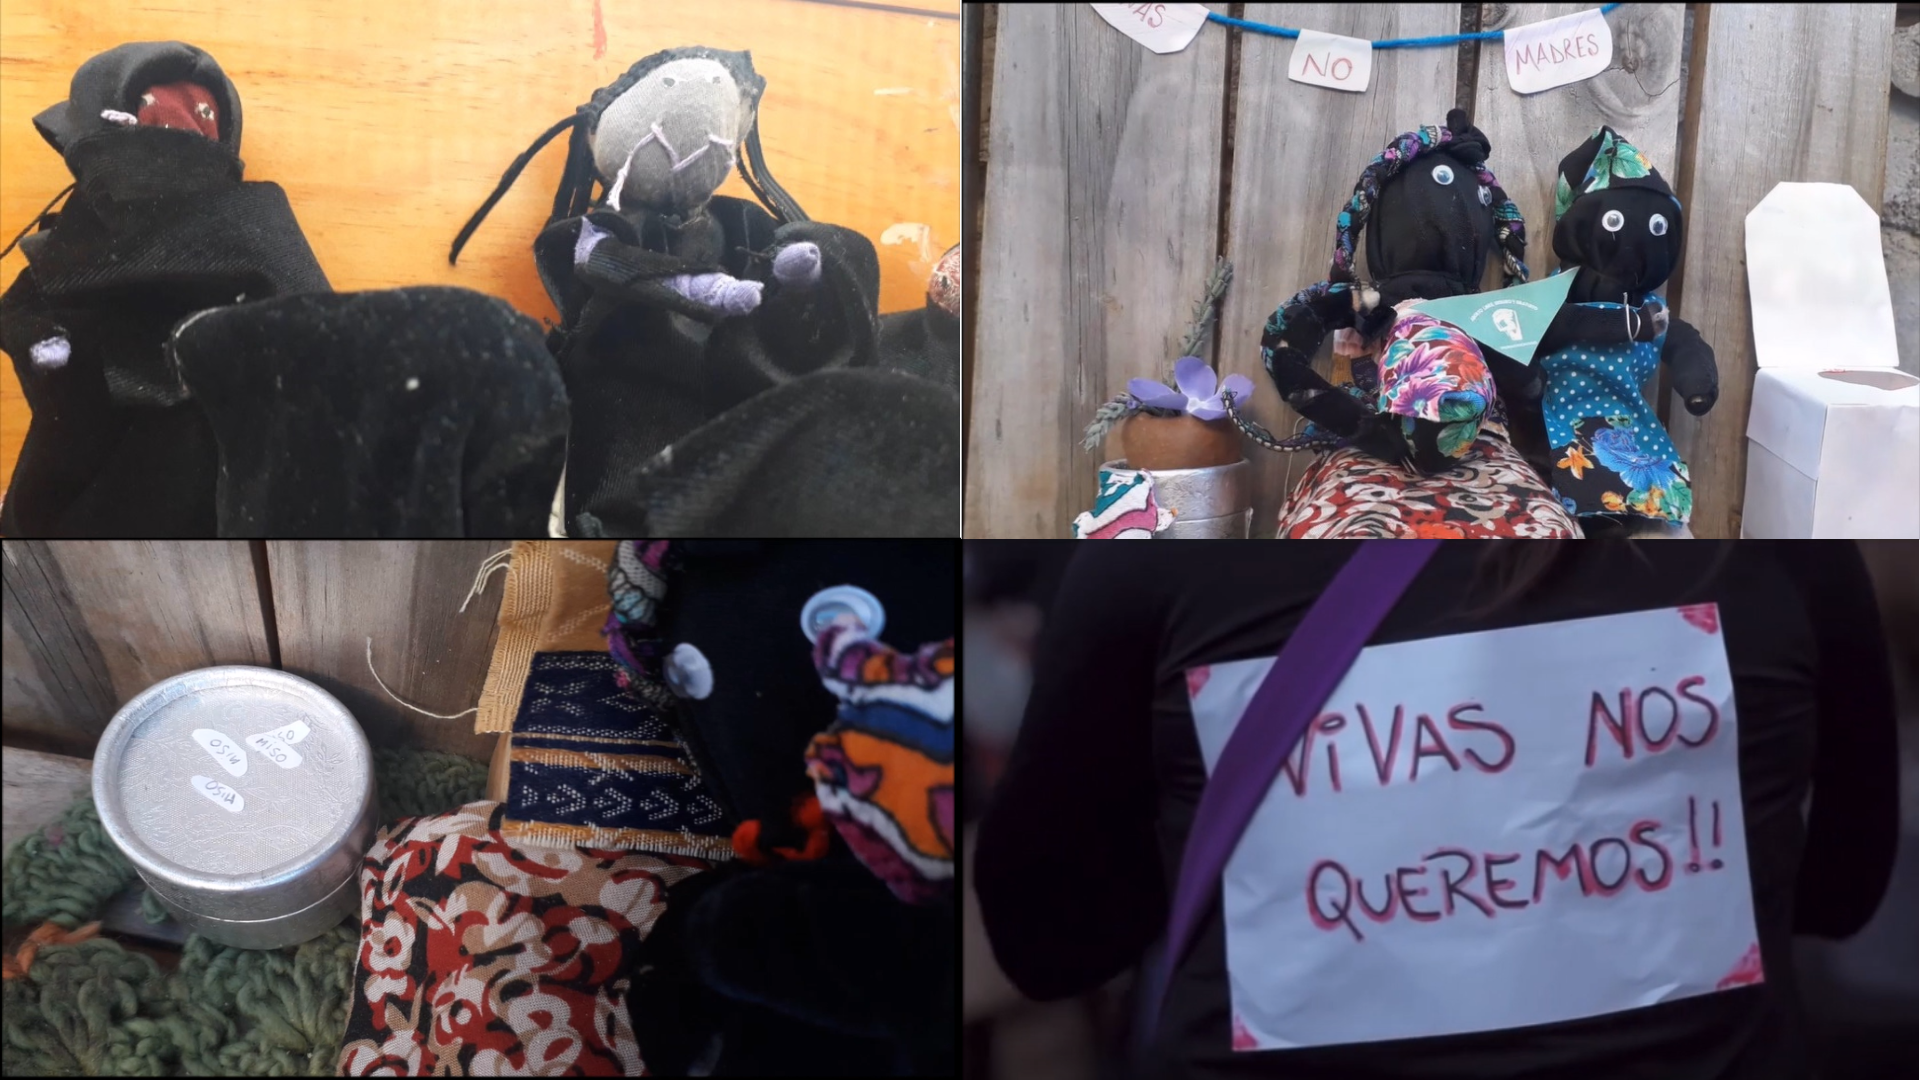
\includegraphics[width=\textwidth]{Fig1.png}
 \caption{Narrativa Transmedia Gladys.}
 \label{fig01}
 \source{Propiedad de la investigación.}
 \end{minipage}
\end{figure}

Las imágenes descritas permitieron determinar que la activación del intertexto lector, donde confluyen la visión de mundo y los aprendizajes previos del lector, es crucial para desarrollar la adecuada interpretación literaria de una obra \cite{mendoza_fillola_lectura_1995,garagalza_sentido_2014}. 

La segunda función, se vincula al \textbf{establecimiento de relaciones intertextuales}, evidenciadas en el contenido de las NT. Por un lado, las cuatro NT establecen intertextualidad con elementos del cuento “Bocas cosidas”, abordando un tema similar, presentando conflictos narrativos ligados al planteado en el cuento e incorporando personajes y símbolos presentes en él. Lo anterior permite constatar que las docentes identificaron los elementos del cuento cruciales para su interpretación literaria.

Por otro lado, la intertextualidad se estableció con producciones culturales, artísticas y televisivas, cuyo contenido estaba directamente relacionado con la interpretación literaria que formularon del cuento. De lo anterior se concluye que, al momento de incorporar producciones ya existentes a su NT, las docentes deben evaluar si existe una relación de estas con el tema que están abordando, por ende, las relaciones de intertextualidad establecidas funcionan como un indicador del grado de desarrollo de la interpretación literaria. Esta función se refleja en la \Cref{fig02}, correspondiente a la NT de Amelia, con relaciones intertextuales que aluden tanto al hipotexto, mediante el tema, la violencia patriarcal, la incorporación del símbolo de las sábanas manchadas con sangre y el personaje travestido; como a intervenciones culturales, empleando en este caso: \textit{Un violador en tu camino}, cuyo propósito es denunciar la violencia patriarcal: “El patriarcado aún esconde las sábanas manchadas con sangre”. Luego añade a uno de los personajes importantes del cuento, la redentora: “La esperanza está en algunes de elles, hombres para algunos, mujeres para otras, rechazada y repudiada por los hombres, amada por las mujeres: la redentora vendrá a hacer visible el abuso y traer libertad”. Para culminar su NT emplea una imagen de la intervención \textit{Un violador en tu camino} del colectivo Las tesis.

\begin{figure}[htbp]
 \centering
 \begin{minipage}{.85\textwidth}
 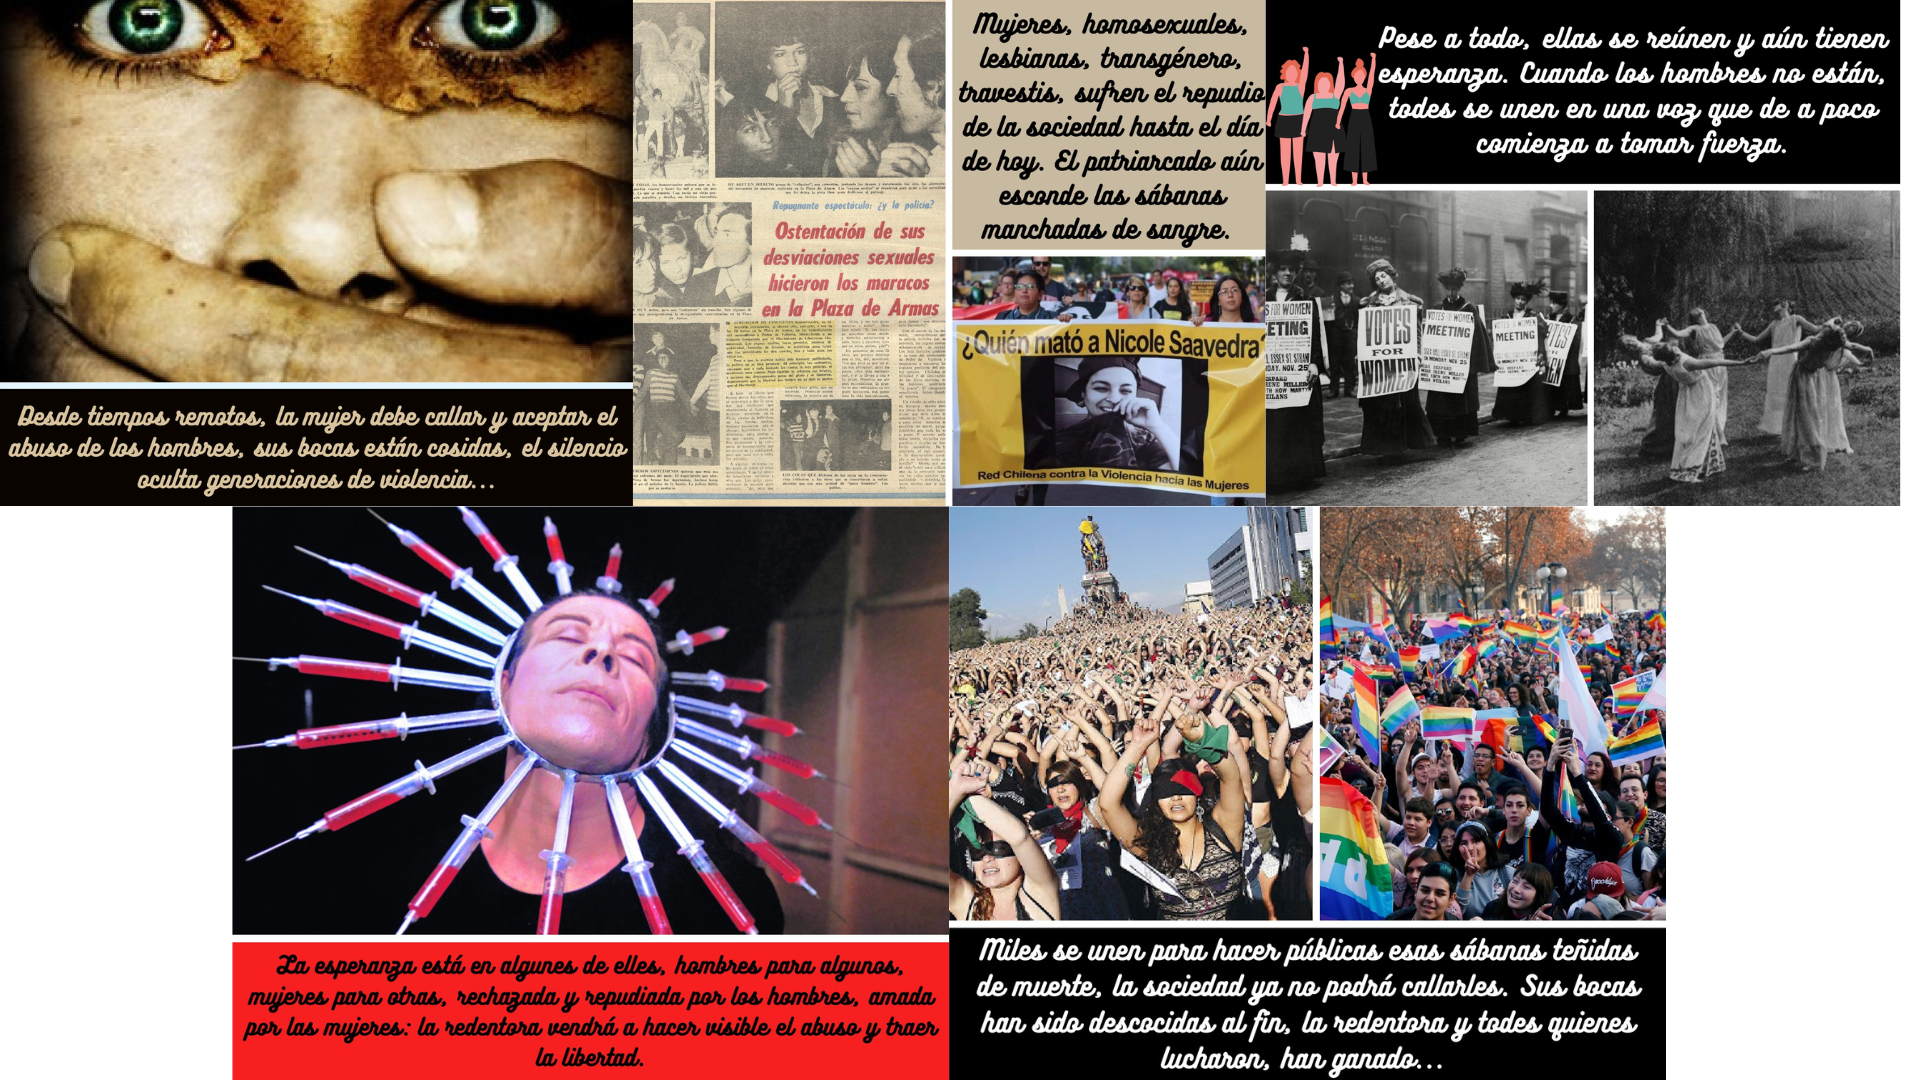
\includegraphics[width=\textwidth]{Fig2.png}
 \caption{Narrativa Transmedia Amelia.}
 \label{fig02}
 \source{Propiedad de la investigación.}
 \end{minipage}
\end{figure}

Otro ejemplo de intertextualidad en las NT de las docentes es la relación que establece con un programa televisivo chileno, \textit{Mujer rompe el silencio} (2003), que se vincula directamente con la temática del texto, en tanto son mujeres que denuncian la violencia a la que han sido sometidas. Emplea el programa para presentar la extensión narrativa del cuento. Luego, en el desarrollo de la NT, aparece el periodista Juan Carlos Bodoque, un personaje de ficción del programa de televisión chileno \textit{31 minutos} que entrevista a una mujer, personaje principal del hipotexto. Para culminar su NT, emplea la canción \textit{Sacar la voz} (2011) de la cantante chilena Anita Tijoux, la cual incentiva la denuncia de los distintos tipos de violencia que se ven en la sociedad. 

\subsection{Interpretación literaria desarrollada a través de las NT}\label{sec-secoes}
Al analizar las producciones, se estudió la interpretación literaria desarrollada a través de las NT, de lo cual se devela que esta se ve reflejada en el \textbf{desenlace} de las cuatro NT, donde aparecen mujeres liberándose de algún tipo de violencia patriarcal, concordando con la interpretación literaria adecuada del cuento “Bocas cosidas”. 

Lo anterior, se plasma en la \Cref{fig03}, correspondiente a la NT de Ester, en la que ella planteó la liberación de las niñas y mujeres de la maternidad obligatoria, visible en la última parte de su producción, en donde aparecen las palabras “MUJERES”, “NIÑAS” y “MADRES”, luego se cambia la palabra “MADRES” por “LIBRES”, quedando así las palabras “NIÑAS” “LIBRES”. Finalmente, la palabra “LIBRES” desaparece y quedan las palabras “NIÑAS”, “no”, “Madre”.

\begin{figure}[htbp]
 \centering
 \begin{minipage}{.65\textwidth}
 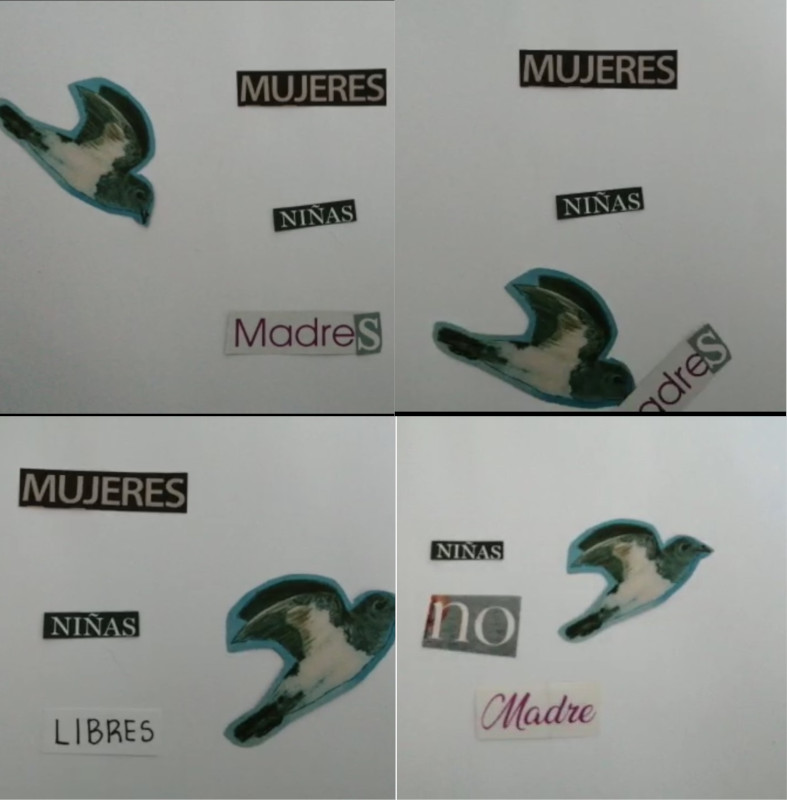
\includegraphics[width=\textwidth]{Fig3.jpg}
 \caption{Narrativa Transmedia Ester.}
 \label{fig03}
 \source{Propiedad de la investigación.}
 \end{minipage}
\end{figure}

En relación con lo expuesto anteriormente, se constata que en la elección del contenido que se emplea para la creación de la NT aparecen indicadores del grado de comprensión e interpretación del texto literario \cite{ramos_estrategias_2008}. En el caso de este estudio las NT presentaron textos, imágenes y audios ligados a aspectos representativos del cuento, dando cuenta de una adecuada interpretación de él.

En cuanto a la definición de NT que hace \textcite{scolari_narrativas_2013} se constata que efectivamente es una práctica de interpretación de la obra que se expresa mediante la combinación de sistemas de significación y distintos formatos, produciendo una nueva creación a partir de la original.

\subsection{Función didáctica de la creación de una NT en el desarrollo de la interpretación literaria}\label{sec-format-simple}
En la última sesión de la SD, emerge la valoración, por parte de las docentes, de la función didáctica de la creación de una NT en el desarrollo de la interpretación literaria, identificando tres beneficios principales de la expansión transmedia: 

El primero está asociado con la\textbf{ planificación de la producción}, ya que esta permite definir y ordenar los elementos del cuento que se emplearán en la NT. Al seleccionarlos y organizarlos para la expansión transmedia, el lector debe evaluar el grado de importancia que tienen en la historia.  

El segundo es consecuencia del primero, dado que el seleccionar y ordenar los aspectos que se tomarán del cuento, permite la \textbf{profundización en los elementos clave} de este para representarlos adecuadamente en la NT, empleando de forma natural, como principal estrategia, la relectura del cuento. 

Finalmente, lo anterior nos lleva al tercer beneficio, al profundizar en los elementos clave del cuento, a través de la relectura, se origina la \textbf{integración del texto al intertexto lector}. Al respecto Tamara comenta: 

\begin{quote}
    Yo creo que sí ayuda a desarrollar una interpretación literaria, sobre todo porque, como que saber que hacia allá tengo que ir, que esa es la meta, implicó que leyera varias veces el texto, como que lo integrara mucho en mí para poder lograr ese producto, entonces, y también estaba, como que uno le podía como impregnar su sello también, entonces eso como que hacía que también uno profundizara también en el texto y a la vez en uno, y la interpretación era mucho más acabada que una pregunta simple en una prueba. (T\_A6\_165\-170)
\end{quote}

El proceso explicado se vincula con lo expuesto por \textcite{cassany_taller_2006} al explicar que la producción conlleva tareas implícitas del proceso lector, como lectura, análisis e interpretación. En consecuencia, la producción aporta y complementa a la comprensión e interpretación literaria de un texto literario.

\section{Conclusiones}\label{sec-links}
El objetivo de este estudio consistía en describir la función didáctica de la expansión transmedia en el desarrollo de la interpretación literaria desde la experiencia de cuatro docentes de lengua y literatura de educación secundaria. Para ello, se realizó un análisis temático a los diferentes productos que emergieron de las sesiones de la SD, a partir del cual se identificaron cuatro temas ligados a los beneficios de la producción de NT para el fortalecimiento de la interpretación literaria. 

El primero corresponde a la expansión narrativa del cuento, estudiada en la planificación de sus NT. Allí se identificó que, en las planificaciones elaboradas por las docentes, tanto el tema, los personajes protagónicos, como los elementos que incluirían en sus producciones se relacionaban con los elementos del cuento leído. El tema predominante en las cuatro planificaciones era la violencia patriarcal, sus personajes principales son mujeres, e incluyeron elementos figurados del cuento, clave para su comprensión. 

El segundo tema se relaciona con la producción digital de la NT, para lo cual las docentes emplearon la transcodificación de sus interpretaciones literarias, utilizando tres sistemas de significación; seleccionaron el contenido de las NT, de lo que se desprenden dos beneficios relevantes, uno vinculado a la activación del intertexto lector, reflejado en la inclusión de elementos de sus conocimientos, ligados a la temática planteada en el texto; y otro asociado a la inclusión de relaciones intertextuales entre sus NT y el cuento leído, como entre las NT con otras producciones culturales que aluden a un tema similar. 

El tercer tema identificado fue la interpretación literaria del cuento leído, cuya adecuación fue determinada por el desenlace propuesto en las cuatro NT, los cuales dan cuenta de la liberación de la mujer del sistema patriarcal que las oprime, conclusión del cuento “Bocas cosidas”, dando cuenta de que el sentido que atribuyeron las docentes al texto fue el adecuado. 

El cuarto tema reconocido en el grupo de enfoque realizado con las docentes fue la función didáctica de la creación de una NT en el desarrollo de interpretación literaria, en donde las profesoras identificaron tres beneficios de la actividad. Uno asociado a la planificación de la producción, que permite definir y ordenar los elementos del cuento que se emplearán en la NT; lo cual conlleva al segundo beneficio, profundizar en estos elementos para poder representarlos adecuadamente en la NT, para lo cual se debe releer el texto, desembocando en el tercer beneficio, que el lector recuerde el texto y lo integre a su intertexto lector.  

De esta manera, el ejercicio desarrollado en la SD fue valorado positivamente por las docentes, quienes manifestaron que efectivamente promueve el desarrollo de la interpretación literaria, pues a través de las relaciones de intertextualidad que establece con otras producciones y de las alusiones a su intertexto lector, reflejadas en el contenido de la NT, se puede medir el grado de relación de este con el sentido del texto, por lo cual podría funcionar como indicador del grado de desarrollo de la interpretación literaria. 

Ahora bien, a pesar de los beneficios asociados a la expansión transmedia para el desarrollo de la expansión literaria, las docentes manifestaron dificultad en su ejecución debido a la carencia de desarrollo de su competencia digital, específicamente en lo que concierne al manejo de las TIC para la creación de contenidos, dificultad que podría limitar la correcta transposición de la interpretación literaria de la obra.

Respecto de las limitaciones del estudio se identifica la pandemia producto de la Covid-19, que imposibilitó que la SD fuese aplicada a estudiantes como estaba determinado en primera instancia. Asimismo, se identifica la imposibilidad de establecer si el grado de desarrollo de la competencia digital de las docentes influenció la pertenencia de la expansión transmedia realizada de la interpretación literaria del cuento leído.

En cuanto a las proyecciones de esta investigación, sería pertinente incorporar al estudiantado como participantes de esta SD, con el fin de evaluar si el ejercicio de expansión transmedia de una obra literaria los ayuda a desarrollar la habilidad de interpretación literaria, y si el grado de desarrollo de las habilidades de alfabetización digital determina la interpretación literaria reflejada en sus producciones transmedia. 


\printbibliography\label{sec-bib}
% if the text is not in Portuguese, it might be necessary to use the code below instead to print the correct ABNT abbreviations [s.n.], [s.l.]
%\begin{portuguese}
%\printbibliography[title={Bibliography}]
%\end{portuguese}


%full list: conceptualization,datacuration,formalanalysis,funding,investigation,methodology,projadm,resources,software,supervision,validation,visualization,writing,review
\begin{contributors}[sec-contributors]
\authorcontribution{Angélica Montaner Henríquez}[conceptualization,datacuration,formalanalysis,investigation,methodology,writing,review]
\authorcontribution{Alba Ambrós-Pallarés}[conceptualization,supervision,writing,review]
\end{contributors}



\end{document}

